\documentclass[12pt]{article}
\usepackage{amsmath}
\usepackage{physics}
\usepackage{mhchem}
\usepackage{tikz}
\usetikzlibrary{positioning}
\author{Patryk Kozlowski}
\title{Problem Set 4}
\date{\today}
\begin{document}
\maketitle
\section{}
\subsection{}
\subsubsection{Question}
Calculate the following matrix element: $\langle l, m+2| (L_x)^2|l,m \rangle$.
\subsubsection{Answer}
The angular momentum raising and lowering operators are given by:
\begin{align*}
L_{\pm} &= L_x \pm iL_y
\end{align*}
We can use these operators to write the following:
\begin{align*}
(L_x)^2 &= \frac{1}{2}(L_+ + L_-)^2\\
&= \frac{1}{2}(L_+^2 + L_-^2 + L_+L_- + L_-L_+)\\
\end{align*}
Now, we recognize that all but the first term will vanish from our matrix element due to orthonormality. So, the original matrix element becomes:
\begin{equation}
\langle l, m+2| (L_x)^2|l,m \rangle = \frac{1}{2}\langle l, m+2| L_+^2|l,m \rangle
\end{equation}
Now, the raising operator acts on a state:
\begin{align*}
L_+|l,m \rangle &= \hbar \sqrt{l(l+1)-m(m+1)}|l,m+1 \rangle
\end{align*}
So, we can write the matrix element as:
\begin{align*}
\langle l, m+2| (L_x)^2|l,m \rangle &= \frac{1}{2}\langle l, m+2| L_+^2|l,m \rangle\\
&= \frac{1}{2}\hbar \sqrt{l(l+1)-m(m+1)}\langle l, m+2| L_+ |l,m+1 \rangle\\
\end{align*}
Now, we can use the raising operator again:
\begin{align*}
L_+|l,m+1 \rangle &= \hbar \sqrt{l(l+1)-(m+1)(m+2)}|l,m+2 \rangle
\end{align*}
So, we can write the matrix element as:
\begin{align*}
\langle l, m+2| (L_x)^2|l,m \rangle &= \frac{1}{2}\hbar \sqrt{l(l+1)-m(m+1)}\langle l, m+2| L_+ |l,m+1 \rangle\\
&= \frac{\hbar ^2}{2}\sqrt{l(l+1)-m(m+1)} \sqrt{l(l+1)-(m+1)(m+2)}\langle l, m+2|l,m+2 \rangle\\
\end{align*}
Assuming orthonormality, we can write the final result as:
\begin{align*}
\langle l, m+2| (L_x)^2|l,m \rangle &= \frac{\hbar ^2}{2}\sqrt{l(l+1)-m(m+1)} \sqrt{l(l+1)-(m+1)(m+2)}\\
\end{align*}
\subsection{}
\subsubsection{Question}
A particle moves in a three-dimensional potential $V(x,y,z)$ that satisfies the commutators $[L_y,V]=0$ and $[L_z,V]=0$. Prove that $[L_x,V]=0$. What does this mean intuitively about the potential?
\subsubsection{Answer}
Since $L_y= xp_z-zp_x$ and $L_z=yp_x-xp_y$, we can write the commutators as:
\begin{align*}
[xp_z-zp_x,V] &= 0\\
[yp_x-xp_y,V] &= 0
\end{align*}
We know that:
\begin{align*}
[xp_z-zp_x,V] &= (xp_z-zp_x)V - V(xp_z-zp_x) = 0\\
\end{align*}
To always be true, we need:
\begin{align*}
xp_zV &= Vxp_z\\
zp_xV &= Vzp_x
\end{align*}
etc. So,
\begin{align*}
Vxp_x &= xVp_x=xp_xV\\
Vzp_z &= zVp_z=zp_zV
\end{align*}
From this, we get the following commutation relations:
\begin{align*}
[x,V]&=0\\
[z,V]&=0\\
[p_x,V]&=0\\
[p_z,V]&=0\\
\end{align*}
Similarly, from the other equation, we get:
\begin{align*}
[y,V]&=0\\
[p_y,V]&=0\\
\end{align*}
So, we can write the following:
\begin{align*}
[L_x, V] &= [yp_z-zp_y, V] &= [yp_z, V]-[zp_y,V]\\
&= y[p_z,V]+[y,V]p_z - z[p_y,V]-[z,V]p_y\\
&= 0
\end{align*}
Everything equals 0 because of the elementary commutators we previously derived.
This means that the potential is "flat," e.g. any change in the x, y, or z direction does not change the respective angular momentum operators.
\subsection{}
\subsubsection{Question}
The matrix's representation of $L_x$ for spin 1 is:
\begin{equation}
L_x = \frac{\hbar}{\sqrt{2}}\begin{pmatrix}
0 & 1 & 0\\
1 & 0 & 1\\
0 & 1 & 0
\end{pmatrix}
\end{equation}
Find the eigenvector of $L_x$ that correspond to the zero eval.
\subsubsection{Answer}
We can do the following system of equations:
\begin{align*}
\frac{\hbar}{\sqrt{2}}\begin{pmatrix}
0 & 1 & 0\\
1 & 0 & 1\\
0 & 1 & 0
\end{pmatrix}\begin{pmatrix}
a\\
b\\
c
\end{pmatrix} &= 0\\
\begin{pmatrix}
b\\
a+c\\
b
\end{pmatrix} &= 0\\
\end{align*}
So, we get the following:
\begin{align*}
b &= 0\\
a+c &= 0\rightarrow a=-c\\
\end{align*}
Then we also have the normalization condition:
\begin{align*}
a^2+b^2+c^2 &= 1\\
a^2+c^2 &= 1\\
2a^2 &= 1\\
a^2 &= \frac{1}{2}\\
a &= \pm \frac{1}{\sqrt{2}}\\
c &= \mp \frac{1}{\sqrt{2}}\\
\end{align*}
So, we get the following eigenvectors:
\begin{align*}
\begin{pmatrix}
\pm\frac{1}{\sqrt{2}}\\
0\\
\mp\frac{1}{\sqrt{2}}
\end{pmatrix}
\end{align*}
It is also worth noting that 0 as an eigenvector is also a trivial solution here, but then the particle would not exist.
\subsubsection{Question}
For an angular momentum 1 particle with 
\begin{equation}
\ket{\psi} = \frac{1}{3}
\begin{pmatrix}
2\\
1\\
-2
\end{pmatrix}
\end{equation}
what is the probability that a measurement of $L_x$ will yield 0, as in what is $|<L_x=0|\psi>|^2$?
\subsubsection{Answer}
We can write the following:
\begin{align*}
|<L_x=0|\psi>|^2 &= |\frac{1}{3\sqrt{2}}\begin{pmatrix}
1 & 0 & -1
\end{pmatrix}\begin{pmatrix}
2\\
1\\
-2
\end{pmatrix}|^2\\
&= |\frac{1}{3\sqrt{2}}(2+2)|^2\\
&= |\frac{4}{3\sqrt{2}}|^2\\
&= \frac{16}{18}\\
&= \frac{8}{9}
\end{align*}


\section{}

\subsection{}
We have $L=2$ and $S=\frac{3}{2}$. So the outer product $L\otimes S$ has the possible values for $J_{\text{tot}}$:
\begin{align*}
J_{\text{tot}} &= L+S = \frac{7}{2}\\
J_{\text{tot}} &= L+S-1 = \frac{5}{2}\\
J_{\text{tot}} &= L+S-2 = \frac{3}{2}\\
J_{\text{tot}} &= L+S-3 = \frac{1}{2}
\end{align*}
\subsection{}
\subsubsection{Question}
Describe each of the possible states with spectroscopic notation.
\subsubsection{Answer}
\begin{align*}
J_{\text{tot}} &= \frac{7}{2} 
\rightarrow \ce{^{4}D_{\frac{7}{2}}}
\\
J_{\text{tot}} &= \frac{5}{2}
\rightarrow \ce{^{4}D_{\frac{5}{2}}}
\\
J_{\text{tot}} &= \frac{3}{2}
\rightarrow \ce{^{4}D_{\frac{3}{2}}}
\\
J_{\text{tot}} &= \frac{1}{2}
\rightarrow \ce{^{4}D_{\frac{1}{2}}}
\end{align*}
\subsection{}
\subsubsection{Question}
Now, imagine that we apply a strong magnetic field to our particle. Magnetic fields couple with angular momentum, allowing for degeneracy to be fully broken. In this case, we will assume that lower values of $J$ correspond to lower energies. Draw an energy level diagram for this system in the presence of a magnetic field and specify each state with its spectroscopic label.
\subsubsection{Answer}
\begin{center}
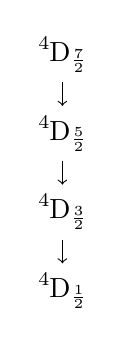
\begin{tikzpicture}
\node (1) at (0,0) {$\ce{^{4}D_{\frac{7}{2}}}$};
\node (2) at (0,-1) {$\ce{^{4}D_{\frac{5}{2}}}$};
\node (3) at (0,-2) {$\ce{^{4}D_{\frac{3}{2}}}$};
\node (4) at (0,-3) {$\ce{^{4}D_{\frac{1}{2}}}$};
\draw[->] (1) -- (2);
\draw[->] (2) -- (3);
\draw[->] (3) -- (4);
\end{tikzpicture}
\end{center}
\section{}
\subsubsection{Question}
This problem will show that there is not a coordinate space representation of spin one half. In other words, there are no spherical harmonics corresponding to spin one half. This is why spin is talked about as an internal degree of freedom, with the total angular momentum being $J=L+S$.
\subsection{}
\subsubsection{Question}
Show that $L_+ \ket{\frac{1}{2},\frac{1}{2}} = 0$ and $L_- \ket{\frac{1}{2},-\frac{1}{2}} = 0$.
\subsubsection{Answer}
We can write the following:
\begin{align*}
L_+ \ket{\frac{1}{2},\frac{1}{2}} &= \hbar \sqrt{\frac{1}{2}(\frac{1}{2}+1)-\frac{1}{2}(\frac{1}{2}+1)}\ket{\frac{1}{2},\frac{1}{2}+1}\\
&= \hbar \sqrt{\frac{1}{2}(\frac{3}{2}) - \frac{1}{2}(\frac{3}{2})}\ket{\frac{1}{2},\frac{1}{2}+1}\\
&= \hbar \sqrt{0}\ket{\frac{1}{2},\frac{1}{2}+1}\\
&= 0
\end{align*}
Similarly, we can write the following:
\begin{align*}
L_- \ket{\frac{1}{2},-\frac{1}{2}} &= \hbar \sqrt{\frac{1}{2}(\frac{1}{2}+1)-(-\frac{1}{2})(-\frac{1}{2}-1)}\ket{\frac{1}{2},-\frac{1}{2}-1}\\
&= \hbar \sqrt{0}\ket{\frac{1}{2},-\frac{1}{2}-1}\\
&= 0
\end{align*}
\subsection{}
\subsubsection{Question}
From the coordinate space representation of the raising and lowering operators, we expect that:
\begin{equation}
    \hbar e^{i\phi}(\frac{\partial}{\partial \theta} + i\cot(\theta)\frac{\partial}{\partial \phi})Y_{\frac{1}{2}}^{\frac{1}{2}}(\theta,\phi) = 0
\end{equation}
and 
\begin{equation}
    \hbar e^{-i\phi}(-\frac{\partial}{\partial \theta} + i\cot(\theta)\frac{\partial}{\partial \phi})Y_{\frac{1}{2}}^{\frac{-1}{2}}(\theta,\phi) = 0
\end{equation}
To be eigenfunctions of $l_z$ the state must have a $\phi$ dependence of $e^{i\phi}$ and $e^{-i\phi}$ respectively. Show that the solutions are $Y_{\frac{1}{2}}^{\frac{1}{2}}(\theta,\phi) = A (\sin(\theta))^{\frac{1}{2}}e^{\frac{i\phi}{2}}$ and $Y_{\frac{1}{2}}^{\frac{-1}{2}}(\theta,\phi) = B (\sin(\theta))^{\frac{1}{2}}e^{-\frac{i\phi}{2}}$.
\subsubsection{Answer}
We can write the following:
\begin{align*}
    \hbar e^{i\phi}(\frac{\partial}{\partial \theta} + i\cot(\theta)\frac{\partial}{\partial \phi})Y_{\frac{1}{2}}^{\frac{1}{2}}(\theta,\phi) &= 0\\
    \hbar e^{i\phi}(\frac{\partial}{\partial \theta} + i\cot(\theta)\frac{\partial}{\partial \phi})A (\sin(\theta))^{\frac{1}{2}}e^{\frac{i\phi}{2}} &= 0\\
    \hbar e^{i\phi}A (\frac{1}{2}(\sin(\theta))^{-\frac{1}{2}}\cos(\theta)e^{\frac{i\phi}{2}} + i\cot(\theta)(\sin(\theta))^{\frac{1}{2}}e^{\frac{i\phi}{2}}\frac{i}{2}) &= 0\\
    \hbar e^{i\phi}A (\frac{1}{2}(\sin(\theta))^{-\frac{1}{2}}\cos(\theta)e^{\frac{i\phi}{2}} - \frac{1}{2}\cos(\theta )( \sin(\theta))^{-\frac{1}{2}}e^{\frac{i\phi}{2}}) &= 0\\
\end{align*}
The term in the parentheses cancels out, so we arrive at
\begin{equation}
    L_+ \ket{\frac{1}{2},\frac{1}{2}} = L_+ Y_{\frac{1}{2}}^{\frac{1}{2}}(\theta,\phi) = 0
\end{equation}
Similarly, we can write the following:
\begin{align*}
    \hbar e^{-i\phi}(-\frac{\partial}{\partial \theta} + i\cot(\theta)\frac{\partial}{\partial \phi})Y_{\frac{1}{2}}^{\frac{-1}{2}}(\theta,\phi) &= 0\\
    \hbar e^{-i\phi}(-\frac{\partial}{\partial \theta} + i\cot(\theta)\frac{\partial}{\partial \phi})B (\sin(\theta))^{\frac{1}{2}}e^{-\frac{i\phi}{2}} &= 0\\
    \hbar e^{-i\phi}B (-\frac{1}{2}(\sin(\theta))^{-\frac{1}{2}}\cos(\theta)e^{-\frac{i\phi}{2}} + i\cot(\theta)(\sin(\theta))^{\frac{1}{2}}e^{-\frac{i\phi}{2}}(-\frac{i}{2})) &= 0\\
    \hbar e^{-i\phi}B (-\frac{1}{2}(\sin(\theta))^{-\frac{1}{2}}\cos(\theta)e^{-\frac{i\phi}{2}} + \frac{1}{2}\cos(\theta )(\sin(\theta))^{-\frac{1}{2}}e^{-\frac{i\phi}{2}}) &= 0\\
\end{align*}
The term in the parentheses cancels out, so we arrive at
\begin{equation}
    L_- \ket{\frac{1}{2},-\frac{1}{2}} = L_- Y_{\frac{1}{2}}^{\frac{-1}{2}}(\theta,\phi) = 0
\end{equation}
\subsection{}
\subsubsection{Question}
The answers in part a look fine, but unfortunately they are not consistent with two more results, namely that $L_+ \ket{\frac{1}{2},-\frac{1}{2}} = \hbar \ket{\frac{1}{2},\frac{1}{2}}$ and $L_- \ket{\frac{1}{2},\frac{1}{2}} = \hbar \ket{\frac{1}{2},-\frac{1}{2}}$. Starting from $Y_{\frac{1}{2}}^{\frac{1}{2}}(\theta,\phi)$ the lowering operator should give $Y_{\frac{1}{2}}^{\frac{-1}{2}}(\theta,\phi)$, and vice versa. Show that
\begin{equation}
    L_- Y_{\frac{1}{2}}^{\frac{1}{2}}(\theta,\phi) = - \hbar A \frac{\cos(\theta )}{\sqrt{\sin(\theta)}}e^{-\frac{i\phi}{2}}
\end{equation}
The rhs is not equal to $Y_{\frac{1}{2}}^{\frac{-1}{2}}(\theta,\phi)$; in fact, it is infinite at $\theta = 0,\pi $. The same can be shown for the raising operator. In other words, no set of spherical harmonics exist for spin one half.
\subsubsection{Answer}
We can write the following:
\begin{align*}
    L_- Y_{\frac{1}{2}}^{\frac{1}{2}}(\theta,\phi) &= \hbar e^{-i\phi}(-\frac{\partial}{\partial \theta} + i\cot(\theta)\frac{\partial}{\partial \phi})A (\sin(\theta))^{\frac{1}{2}}e^{\frac{i\phi}{2}}\\
    &= \hbar A e^{-i\phi} (-\frac{1}{2}(\sin(\theta))^{-\frac{1}{2}}\cos(\theta)e^{\frac{i\phi}{2}} + i\cot(\theta)(\sin(\theta))^{\frac{1}{2}}e^{\frac{i\phi}{2}}\frac{i}{2})\\
    &= -\hbar A e^{-\frac{i \phi}{2}} (\frac{1}{2}(\sin(\theta))^{-\frac{1}{2}}\cos(\theta) + \frac{1}{2}(\cos(\theta )\sin(\theta))^{-\frac{1}{2}})\\
    &= -\hbar A \frac{\cos(\theta )}{\sqrt{\sin(\theta)}}e^{-\frac{i\phi}{2}}
\end{align*}
\end{document}